%%%%%%%%%%%%%%%%%%%%%%%%%%%%%%%%%%%%%%%%%
% Beamer Presentation
% LaTeX Template
% Version 1.0 (10/11/12)
%
% This template has been downloaded from:
% http://www.LaTeXTemplates.com
%
% License:
% CC BY-NC-SA 3.0 (http://creativecommons.org/licenses/by-nc-sa/3.0/)
%
%%%%%%%%%%%%%%%%%%%%%%%%%%%%%%%%%%%%%%%%%

%----------------------------------------------------------------------------------------
%	PACKAGES AND THEMES
%----------------------------------------------------------------------------------------

\documentclass[handout]{beamer}

\mode<presentation> {

% The Beamer class comes with a number of default slide themes
% which change the colors and layouts of slides. Below this is a list
% of all the themes, uncomment each in turn to see what they look like.

%\usetheme{default}
%\usetheme{AnnArbor}
%\usetheme{Antibes}
%\usetheme{Bergen}
%\usetheme{Berkeley}
%\usetheme{Berlin}
%\usetheme{Boadilla}
%\usetheme{CambridgeUS}
%\usetheme{Copenhagen}
%\usetheme{Darmstadt}
%\usetheme{Dresden}
%\usetheme{Frankfurt}
%\usetheme{Goettingen}
%\usetheme{Hannover}
%\usetheme{Ilmenau}
%\usetheme{JuanLesPins}
%\usetheme{Luebeck}
\usetheme{Madrid}
%\usetheme{Malmoe}
%\usetheme{Marburg}
%\usetheme{Montpellier}
%\usetheme{PaloAlto}
%\usetheme{Pittsburgh}
%\usetheme{Rochester}
%\usetheme{Singapore}
%\usetheme{Szeged}
%\usetheme{Warsaw}

% As well as themes, the Beamer class has a number of color themes
% for any slide theme. Uncomment each of these in turn to see how it
% changes the colors of your current slide theme.

%\usecolortheme{albatross}
%\usecolortheme{beaver}
%\usecolortheme{beetle}
%\usecolortheme{crane}
%\usecolortheme{dolphin}
%\usecolortheme{dove}
%\usecolortheme{fly}
%\usecolortheme{lily}
%\usecolortheme{orchid}
%\usecolortheme{rose}
%\usecolortheme{seagull}
%\usecolortheme{seahorse}
%\usecolortheme{whale}
%\usecolortheme{wolverine}

%\setbeamertemplate{footline} % To remove the footer line in all slides uncomment this line
%\setbeamertemplate{footline}[page number] % To replace the footer line in all slides with a simple slide count uncomment this line

%\setbeamertemplate{navigation symbols}{} % To remove the navigation symbols from the bottom of all slides uncomment this line
}

\usepackage{graphicx} % Allows including images
\usepackage{booktabs} % Allows the use of \toprule, \midrule and \bottomrule in tables
\usepackage{cool}
\usepackage{tikz}
\usepackage{amsmath}
\usepackage{pseudocode}
\usepackage{MnSymbol,wasysym}
\DeclareMathOperator*{\argmax}{argmax}
\DeclareMathOperator*{\argmin}{argmin}
\usetikzlibrary{positioning}

%----------------------------------------------------------------------------------------
%	TITLE PAGE
%----------------------------------------------------------------------------------------

\title[Blending Learning and Planning Chapter]{A Guided Tour of \href{http://stanford.edu/~ashlearn/RLForFinanceBook/book.pdf}{\underline{\textcolor{yellow}{Chapter 16}}}: \\ Blending Learning and Planning} % The short title appears at the bottom of every slide, the full title is only on the title page

\author{Ashwin Rao} % Your name
\institute[Stanford] % Your institution as it will appear on the bottom of every slide, may be shorthand to save space
{
ICME, Stanford University
}

\date{\today} % Date, can be changed to a custom date


\begin{document}
\begin{frame}
\titlepage % Print the title page as the first slide
\end{frame}

\begin{frame}
\frametitle{Planning versus Learning}
\pause
\begin{itemize}[<+->]
\item {\em Planning} and {\em Learning} refer to two different AI methodologies
\item Let's understand what they mean for MDP Prediction and Control
\item AI Agent has access to an MDP Environment $E$
\item By interacting with $E$, AI Agent receives experiences data
\item Goal is to estimate requisite VF/Policy using these experiences
\item Broadly, there are two ways to do this:
\begin{itemize}[<+->]
\item {\em Planning} (Model-based approach): Build a model $M$ from interaction experiences, then use $M$ to estimate requisite VF/Policy
\item {\em Learning} (Model-free approach): Don't bother with a model, use interaction experiences to directly estimate VF/Policy (with RL)
\end{itemize}
\end{itemize}
\end{frame}


\begin{frame}
\frametitle{Two different approaches to {\em Planning}}
\pause
\begin{itemize}[<+->]
\item Building model $M$ from experiences data is Supervised Learning
\item Then estimate requisite VF/Policy using model $M$
\item There are two different approaches to estimate VF/Policy from $M$
\item The first approach is to build an explicit representation of  $\mathcal{P}_R$
\item Then employ Dynamic Programming or Tree-Search
\item This approach doesn't require interactions with $E$ (since we have $M$)
\item The second approach is to build a sampling model of $\mathcal{P}_R$
\item Sampling model gives us a Simulated Environment $S$
\item Now interact with $S$ (instead of $E$) and solve VF/Policy using RL
\item This approach is known as Model-based RL
\end{itemize}
\end{frame}

\begin{frame}
\frametitle{Planning with a Supervised-Learnt Model}
\pause
\begin{figure}
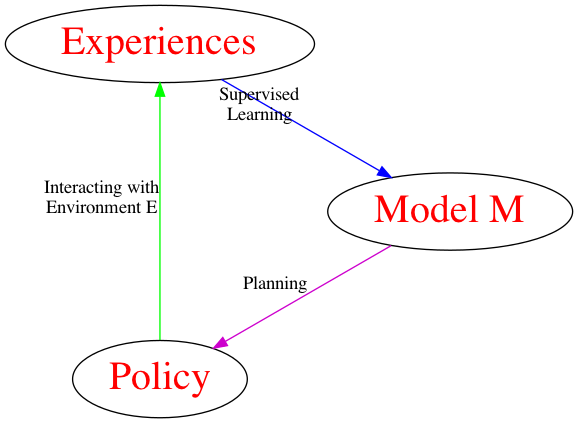
\includegraphics[scale=0.5]{planning.png}
\end{figure}
\end{frame}

\begin{frame}
\frametitle{Blending Planning and Learning}
\pause
\begin{figure}
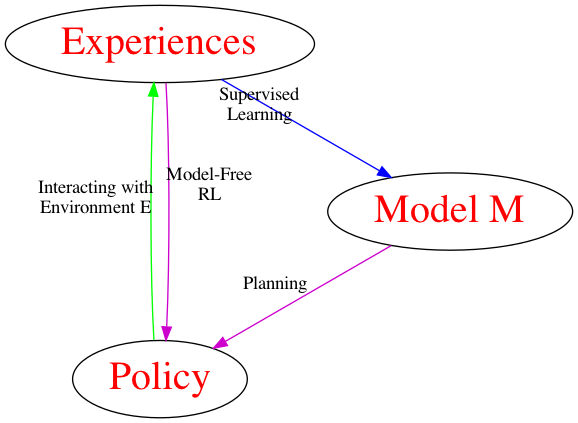
\includegraphics[scale=0.5]{planning_learning.png}
\end{figure}
\end{frame}

\begin{frame}
\frametitle{Decision-Time Planning}
\pause
\begin{itemize}[<+->]
\item {\em Background Planning}:  Pre-compute requisite VF/Policy {\em for all states}
\item So when it's time to perform an action for a given state, just refer to pre-computed Policy
\item In the {\em background}, the VF/Policy  is being constantly improved (irrespective of which state is to be acted on)
\item {\em Decision-Time Planning}: The calculations to identify the best action for a state are started only upon reaching that state
\item Do this when too many states make Background Planning infeasible
\item However, this means we need sufficient time to perform the calculations to identify the best action upon reaching a specific state
\item Decision-Time Planning typically looks deeper than a time step ahead
\item By growing out a tree of future states/actions/rewards
\item Tree rooted at the state of current interest (where the entire focus is)
\end{itemize}
\end{frame}



\begin{frame}
\frametitle{Monte Carlo Tree Search (MCTS)}
\pause
\begin{itemize}[<+->]
\item MCTS was popularized a few years ago by \href{https://www.nature.com/articles/nature16961}{\underline{\textcolor{blue}{Deep Mind's AlphaGo}}}
\item It is a simulation-based method to identify the best action in a state
\item MCTS term was first introduced by \href{https://hal.inria.fr/inria-00116992/document}{\underline{\textcolor{blue}{Remi Coulom}}} for game trees
\item Each round of MCTS consists of four steps:
\begin{itemize}
\item Selection: Successively select children from root R to leaf L
\item Expansion: Create node C as a new child of L
\item Simulation: Complete a random playout from C
\item Backpropagation: Use result of playout to update nodes from C to R
\end{itemize}
\end{itemize}
\begin{figure}
\includegraphics[scale=0.115]{MCTS.png}
\end{figure}
\end{frame}

\begin{frame}
\frametitle{The Selection Step in MCTS}
\pause
\begin{itemize}[<+->]
\item Selection involves picking a child with ``most promise''
\item This means prioritizing children with higher success estimates
\item For estimate confidence, we need sufficient playouts under {\em each} child
\item This is our usual {\em Explore v/s Exploit} dilemma (Multi-armed Bandit)
\item Explore v/s Exploit formula for games first due to \href{http://ggp.stanford.edu/readings/uct.pdf}{\underline{\textcolor{blue}{Kocsis-Szepesvari}}}
\item Formula called {\em Upper Confidence Bound 1 for Trees} (abbrev. UCT)
\item Most current MCTS Algorithms are based on some variant of UCT
\item UCT is based on UCB1 formula of \href{https://homes.di.unimi.it/cesa-bianchi/Pubblicazioni/ml-02.pdf}{\underline{\textcolor{blue}{Auer, Cesa-Bianchi, Fischer}}}
\item However, MCTS and UCT concepts first appeared in the \href{https://pdfs.semanticscholar.org/a378/b2895a3e3f6a19cdff1a0ad404b301b5545f.pdf}{\underline{\textcolor{blue}{Adaptive Multistage Sampling algorithm of Chang, Fu, Hu, Marcus}}}
\item Adaptive Multistage Sampling (AMS) is a generic simulation-based algorithm to solve a finite-horizon Markov Decision Process (MDP)
\item AMS can be considered as the ``spiritual origin'' of MCTS/UCT
\item Hence, this lecture is dedicated to AMS
\end{itemize}
\end{frame}

\begin{frame}
\frametitle{The Setting for the AMS Algorithm}
\pause
\begin{itemize}[<+->]
\item MDP with finite number of time steps $t=0, 1, \ldots, T$
\item State denoted $s_t \in \mathcal{S}$, where $\mathcal{S}$ is very large
\item Action denoted $a_t \in \mathcal{A}$, where $\mathcal{A}$ is fairly small
\item Reward $r_t \in \mathbb{R}$, with $\mathbb{E}[r_t|(s_t, a_t)]$ provided as a function $R_t(s_t,a_t)$
\item Next time step's state $s_{t+1}$ can be generated by invoking a random sampling function $SF_t(s_t,a_t)$, i.e., $s_{t+1} = SF_t(s_t, a_t)()$
\item Discount factor denoted as $\gamma$, and $r_T = 0$
\item The problem is to calculate the Optimal Value function $V_t^*(s_t)$
\item Unlike tabular backward induction where state transition probabilities are given, here only a sampling function (for next state) is given
\item Armed with the sampling function, can we do better than backward induction for the case where $\mathcal{S}$ is very large and $\mathcal{A}$ is small?
\end{itemize}
\end{frame}

\begin{frame}
\frametitle{Outline of AMS Algorithm}
\pause
\begin{itemize}[<+->]
\item AMS Algorithm is based on a fixed allocation of action selections for each state in each time step
\item Denote number of action selections per state in time step $t$ as $N_t$
\item Denote $\hat{V}_t^{N_t}(s_t)$ as the AMS Algorithm estimate of $V_t^*(s_t)$
\item Let $N_t^{s_t,a_t}$ be the number of selections of $a_t$ for $s_t$ ($\sum_{a_t \in \mathcal{A}} N_t^{s_t,a_t} = N_t$)
\item Proportions of $N_t^{s_t,a_t}$ based on {Explore v/s Exploit} UCT formula
\item For each of the $N_t^{s_t,a_t}$ selections of $a_t$, {\em one} next-state $s_{t+1}$ is sampled
\item Denote $j$-th sample of $s_{t+1}$ for fixed $s_t,a_t$ as $s_{t+1}^{(s_t,a_t,j)}, j = 1, \ldots, N_t^{s_t,a_t}$
\item Optimal Action Value Function $Q_t^*(s_t, a_t)$ estimated as:
$$\hat{Q}_t^{N_t}(s_t,a_t) = R(s_t,a_t) + \gamma \cdot \frac {\sum_{j=1}^{N_t^{s_t,a_t}} \hat{V}_{t+1}^{N_{t+1}}(s_{t+1}^{(s_t,a_t,j)})} {N_t^{s_t,a_t}}$$
\item $V_t^*(s_t) = \max_{a_t} Q_t^*(s_t,a_t)$ approximated as:
$$\hat{V}_t^{N_t}(s_t) = \sum_{a_t} \frac {N_t^{s_t,a_t}} {N_t} \cdot \hat{Q}_t^{N_t}(s_t,a_t)$$
\end{itemize}
\end{frame}


\begin{frame}
\frametitle{Running Time, Bias, Convergence and Code}
\pause
\begin{itemize}[<+->]
\item Let $N = \max{(N_0, N_1, \ldots, N_{T-1})}$ and assume $N > |\mathcal{A}|$
\item Running time of AMS Algorithm is of the order of $N^T \cdot |\mathcal{A}|$
\item Compare this versus backward induction running time of $|\mathcal{S}|^2 \cdot |\mathcal{A}| \cdot T$
\item So AMS is more efficient when $\mathcal{S}$ is very large (typical in real-world)
\item \href{https://pdfs.semanticscholar.org/a378/b2895a3e3f6a19cdff1a0ad404b301b5545f.pdf}{\underline{\textcolor{blue}{AMS paper}}} proves the estimate $\hat{V}_0^{N_0}(s_0)$ is asymptotically unbiased
$$\lim_{N_0\rightarrow \infty} \lim_{N_1\rightarrow \infty} \ldots \lim_{N_{T-1}\rightarrow \infty} \mathbb{E}[\hat{V}_0^{N_0}(s_0)] = V_0^*(s_0) \mbox{ for all } s_0 \in \mathcal{S}$$
\item AMS paper also proves that the worst-possible bias is bounded by a quantity that converges to zero at rate $O(\sum_{t=0}^{T-1} \frac {\ln N_t} {N_t})$
$$0 \leq V_0^*(s_0) - \mathbb{E}[\hat{V}_0^{N_0}(s_0)] \leq O(\sum_{t=0}^{T-1} \frac {\ln N_t} {N_t}) \mbox{ for all } s_0 \in \mathcal{S}$$
\item Here's some \href{https://github.com/coverdrive/MDP-DP-RL/blob/master/src/algorithms/ams.py}{\underline{\textcolor{blue}{Python code for the AMS Algorithm}}} you can play with
\end{itemize}
\end{frame}


\end{document}